\documentclass[aspectration=1610,t]{beamer}
\usepackage{csc}
\title{Лекция 2. OpenGL --- шейдеры и текстуры}


\date{
   \textbf{ИТМО}\\
   21 сентября 2022\\
   Санкт-Петербург
}

\begin{document}

\begin{frame}
  \titlepage
\end{frame}

\begin{frame}[fragile]{Еще раз о шейдерах}
    Нас интересуют 2 вида шейдеров:
    \begin{itemize}
        \item {\bf вершинный} - обрабатывает каждую вершину геометрии;
        \item {\bf фрагментный} - обрабатывает каждый фрагмент (упрощенно пиксель).
    \end{itemize}

    Типичный шейдер:
            {\small \begin{lstlisting}
#version version_number

in type in_name; // and others
out type out_name; // and maybe others
uniform type uni_name; // and maybe others

void main() {
    out_name = calculations;
}
            \end{lstlisting}}
\end{frame}

\begin{frame}[fragile]{Типы в шейдерах}
    Широкоиспользуемые:
    \begin{itemize}
        \item {\bf int, float, double, uint, bool} - численные значения;
        \item {\bf vec2, vec3, vec4 } - вектора заданной размерности типа float;
        \item {\bf mat2, mat3, mat4, ...} - матрицы заданной размерности, тип float.
        \item {\bf bvecN, ivecN, uvecN, ... } - вектора, заданной размерности, но другого числового типа;
    \end{itemize}
\end{frame}

\begin{frame}[fragile]{Вектора в шейдерах}
    Для векторных типов можно доступаться либо по индексу (не рекомендуется), либо по имени ({\bf xyzw, rgba, stpq }).
    
    Поддерживается swizzling.
            {\small \begin{lstlisting}
void main() {
    vec4 color = vec4(1., 0., 0., 1);
    vec4 other_color = color.argb;

    vec4 pos = vec4(1., 1., 1., 1);
    vec4 other_pos = pos.xxyw; // swizzling

    vec2 tex = vec2(0., 0.5);
    vec3 other_tex = vec3(tex.st, 1.);
}
            \end{lstlisting}}
\end{frame}

\begin{frame}[fragile]{Примеры функций}
    \begin{itemize}
        \item Работа с векторами и матрицами (cross, dot, reflect, normalize, length, ...);
        \item Тригонометрия (sin, cos, tan, asin, radians, degrees, ...);
        \item Математические функции (pow, sqrt, abs, log, ...);
        \item Фильтры (clamp, mix, step, ...);
        \item ...
    \end{itemize}
\end{frame}

\begin{frame}[fragile]{Еще раз о location}
    Для связывания атрибутов из основного кода и значений внутри шейдеров используется {\bf location }).
            {\small \begin{lstlisting}
#version 330 core
layout (location = 0) in vec3 position; // 0
layout (location = 1) in vec4 color; // 1

out vec4 vectex_color; 

void main() {
    vectex_color = vec4(0.5 * color.rgb, color.a);
    gl_Position = vec4(position, 1.0);
}
            \end{lstlisting}}
\end{frame}

\begin{frame}[fragile]{Еще раз о атрибутах}
    Сами данные хранятся как непрерывная последовательность байтов.
    \begin{figure}[htp]
        \centering
        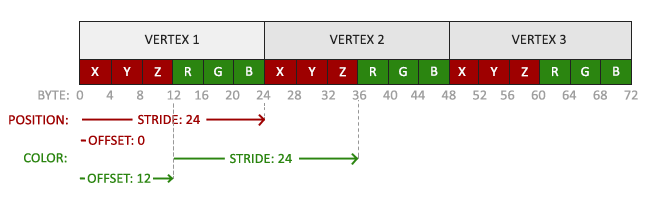
\includegraphics[scale=0.40]{res/attr}
    \end{figure}
\end{frame}

\begin{frame}[fragile]{Еще раз юниформах}
    Пример код на \langcpp:
    {\small \begin{lstlisting}
GLfloat green = (sin(time()) / 2) + 0.5;
GLint loc = glGetUniformLocation(shaderProgram,
                                 "u_color");
glUseProgram(shaderProgram);
glUniform4f(loc, 0.0f, green, 0.0f, 1.0f);
\end{lstlisting}}
    
    Пример шейдер:
    {\small \begin{lstlisting}
#version 330 core
out vec4 color;
uniform vec4 u_color;
void main() {
    color = u_color;
}
    \end{lstlisting}}
\end{frame}

\begin{frame}[fragile]{Текстуры}
    Текстура ~--- это 2D изображение (1D и 3D текстура также существуют), используемое для добавления деталей объекту.

    \begin{figure}[htp]
        \centering
        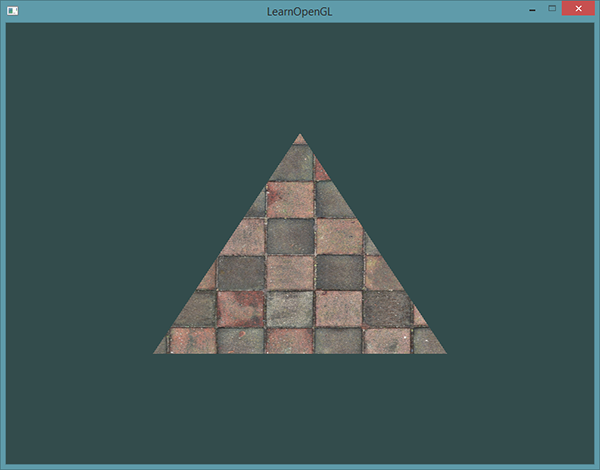
\includegraphics[scale=0.40]{res/tex}
    \end{figure}
\end{frame}

\begin{frame}[fragile]{Текстуры}
    Для того, чтобы привязать текстуру к геометрии используются текстурные координаты.
    \begin{itemize}
        \item Получение цвета из текстуры - сэмплирование ({\bf sampling}).
        \item {\bf u, v} - обозначение, {\bf [0, 1]} - диапазон значений типа float;
    \end{itemize}

    \begin{figure}[htp]
        \centering
        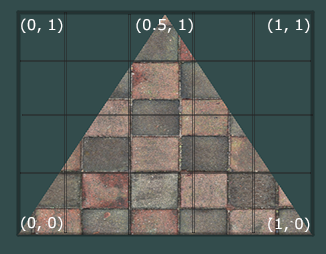
\includegraphics[scale=0.40]{res/tex_coor}
    \end{figure}
\end{frame}

\begin{frame}[fragile]{Texture wrapping}
    Возможно настроить поведение при выходе за диапазон координат.
    \begin{figure}[htp]
        \centering
        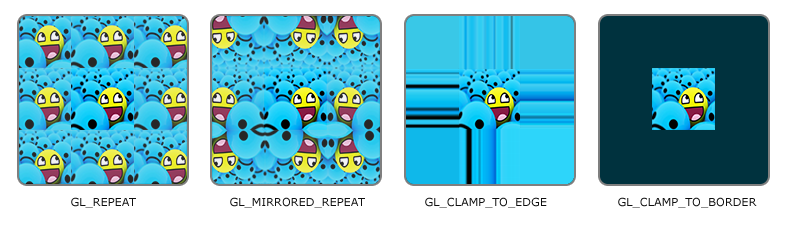
\includegraphics[scale=0.40]{res/tex_wrap}
    \end{figure}

    Код для установки параметров:
    {\small \begin{lstlisting}
glTexParameteri(GL_TEXTURE_2D, GL_TEXTURE_WRAP_S,
                GL_MIRRORED_REPEAT);
glTexParameteri(GL_TEXTURE_2D, GL_TEXTURE_WRAP_T,
                GL_MIRRORED_REPEAT);
    \end{lstlisting}}
\end{frame}

\begin{frame}[fragile]{Texture filtering}
    Текстурные координаты нормализованы и выбор конкретного пикселя (текселя) из текстуры может быть параметризован.
    Существуют различные варианты фильтрации:
    \begin{itemize}
        \item {\bf GL\_NEAREST} - ближайший.
        \item {\bf GL\_LINEAR} - билинейная фильтрация.
    \end{itemize}
\end{frame}

\begin{frame}[fragile]{Texture mipmap}
    Служат для получения текстур меньшего размера. Для генерации существует соответсвующий метод {\bf glGenerateMipmaps}.
    \begin{figure}[htp]
        \centering
        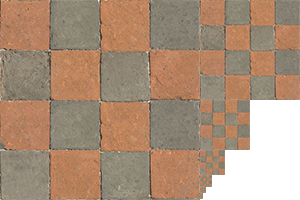
\includegraphics[scale=0.40]{res/tex_mip}
    \end{figure}
    Различные методы фильтрации:
    \begin{itemize}
        \item {\bf GL\_NEARESET\_MIPMAPNEAREST};
        \item {\bf GL\_LINEAR\_MIPMAPNEAREST};
        \item {\bf GL\_NEAREST\_MIPMAPLINEAR}.
    \end{itemize}
\end{frame}

\begin{frame}[fragile]{Texture filtering}
    Различные режимы фильтрации дают различные картинки.
    \begin{figure}[htp]
        \centering
        
\includegraphics[scale=0.40]{res/tex_fil}
    \end{figure}

    Код для установки параметров:
    {\small \begin{lstlisting}
glTexParameteri(GL_TEXTURE_2D, GL_TEXTURE_MIN_FILTER,
                GL_LINEAR);
glTexParameteri(GL_TEXTURE_2D, GL_TEXTURE_MAG_FILTER,
                GL_LINEAR);
    \end{lstlisting}}
\end{frame}

\begin{frame}[fragile]{Загрузка текстуры}
    Генерация текстуры:
    {\small \begin{lstlisting}
GLuint texture;
glGenTextures(1, &texture);
    \end{lstlisting}}
    Заливка в видеопамять:
    {\small \begin{lstlisting}
glBindTexture(GL_TEXTURE_2D, texture);
glTexImage2D(GL_TEXTURE_2D, 0, GL_RGBA, 
             width, height, 0, GL_RGB,
             GL_UNSIGNED_BYTE, image);
glGenerateMipmap(GL_TEXTURE_2D);
glBindTexture(GL_TEXTURE_2D, 0); // use default
    \end{lstlisting}}
\end{frame}

\begin{frame}[fragile]{Передача текстуры в шейдер}
    Сам объект текстуры же передаем как uniform переменную специального типа {\bf sampler2D }.
    {\small \begin{lstlisting}
#version 330 core
in vec2 tex_coord;
out vec4 color;
uniform sampler2D tex_2d;

void main() {
    color = texture(tex_2d, tex_coord);
}
    \end{lstlisting}}
    Текстурные координаты передаем как атрибуты вершин.
\end{frame}

\begin{frame}[fragile]{Передача нескольких текстур}
    По умолчанию используется текстурный блок с индексом 0. Однако есть возможность передать несколько текстур.
    {\small \begin{lstlisting}
// Activate block
glActiveTexture(GL_TEXTURE1);
// Now texture is binded for 1 block
glBindTexture(GL_TEXTURE_2D, texture);
    \end{lstlisting}}
    Всего доступно 16 текстурных блоков {\bf GL\_TEXTURE0, GL\_TEXTURE1, ..., GL\_TEXTURE15}.
\end{frame}

\begin{frame}[fragile]{Передача нескольких текстур}
    Финальный шаг связать наши uniform-переменные и сами текстуры.
    {\small \begin{lstlisting}
glActiveTexture(GL_TEXTURE0);
glBindTexture(GL_TEXTURE_2D, texture1);
glUniform1i(glGetUniformLocation(sp, "tex_2d"), 0);
glActiveTexture(GL_TEXTURE1);
glBindTexture(GL_TEXTURE_2D, texture2);
glUniform1i(glGetUniformLocation(sp, "tex_2d_2"), 1);
    \end{lstlisting}}
\end{frame}

\begin{frame}[fragile]{Передача нескольких текстур}
    Фрагментный шейдер же примет вид:
    {\small \begin{lstlisting}
// ...

uniform sampler2D tex_2d;
uniform sampler2D tex_2d_2;

void main() {
    color = mix(
        texture(tex_2d, tex_coord),
        texture(tex_2d_2, tex_coord), 0.4);
}
    \end{lstlisting}}
\end{frame}

\end{document}

